% 1985 年全国卷理科第 15 题：线段 AB 在 y=x 上移动
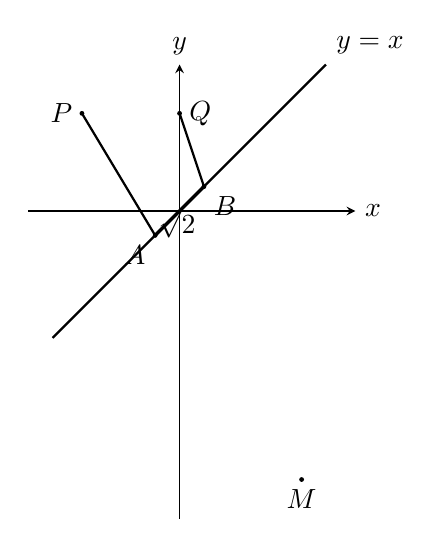
\begin{tikzpicture}[scale=0.62,>=stealth]
  \draw[->] (-3.1,0)--(3.6,0) node[right] {$x$};
  \draw[->] (0,-6.3)--(0,3.0) node[above] {$y$};
  \draw[thick] (-2.6,-2.6)--(3.0,3.0) node[above right] {$y=x$};
  \coordinate (P) at (-2,2);
  \coordinate (Q) at (0,2);
  \coordinate (A) at (-0.5,-0.5);
  \coordinate (B) at (0.5,0.5);
  \coordinate (M) at (2.5,-5.5);
  \draw[thick] (P)--(A);
  \draw[thick] (Q)--(B);
  \draw[very thick] (A)--(B);
  \fill (P) circle (1.4pt) node[left] {$P$};
  \fill (Q) circle (1.4pt) node[right] {$Q$};
  \fill (A) circle (1.4pt) node[below left] {$A$};
  \fill (B) circle (1.4pt) node[below right] {$B$};
  \fill (M) circle (1.4pt) node[below] {$M$};
  \node at (-0.05,-0.25) {$\sqrt2$};
\end{tikzpicture}
